\documentclass[12pt]{article}
\usepackage[margin=0.75in]{geometry} 
\usepackage{amsmath,amsthm,amssymb}
\usepackage{longtable}
\usepackage{mathtools}
\usepackage{standalone}
\usepackage{listings}
\usepackage{array}
\usepackage{float}
\usepackage{verbatim}
\usepackage{caption}
\usepackage{color} %red, green, blue, yellow, cyan, magenta, black, white
\definecolor{mygreen}{RGB}{28,172,0} % color values Red, Green, Blue
\definecolor{mylilas}{RGB}{170,55,241}

\graphicspath{{../}}

% Set parameters for formatting imported Matlab
\lstset{language=Matlab,%
	basicstyle=\small
	%basicstyle=\color{red},
	breaklines=true,%
	morekeywords={matlab2tikz},
	keywordstyle=\color{blue},%
	morekeywords=[2]{1}, keywordstyle=[2]{\color{black}},
	identifierstyle=\color{black},%
	stringstyle=\color{mylilas},
	commentstyle=\color{mygreen},%
	showstringspaces=false,%without this there will be a symbol in the places where there is a space
	numbers=left,%
	numberstyle={\tiny \color{black}},% size of the numbers
	numbersep=9pt, % this defines how far the numbers are from the text
	emph=[1]{for,end,break},emphstyle=[1]\color{red}, %some words to emphasise
	%emph=[2]{word1,word2}, emphstyle=[2]{style},    
}

\title{Image Processing Sensitivity Analysis}
\author{Jack Cole}
\date{}



\begin{document}
\maketitle
\section{Introduction}
What questions are we trying to answer
\subsection{Methods}
How did we try to answer them
\subsection{Results}
Present the results
For example figure \ref{fig:botALeftCol} shows some stuff.
\begin{figure}[H]
	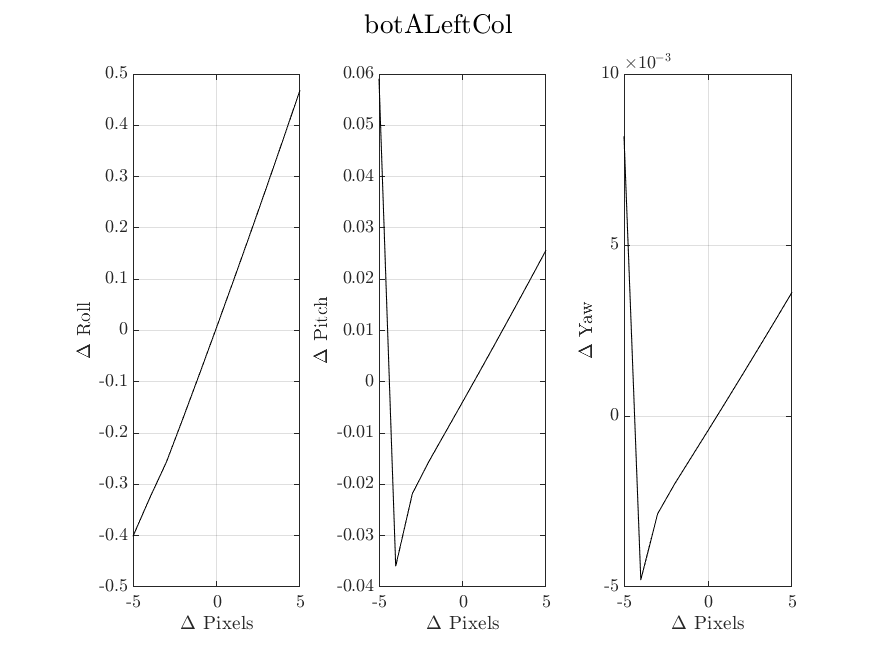
\includegraphics[width=0.9\columnwidth]{botALeftCol.png}
	\caption{Caption here.\label{fig:botALeftCol}}
\end{figure}

\subsection{Discussion}
What conclusions can we draw, specifically: what was as expected, what was not as expected?

\end{document} 
%%%%%%%%%%%%%%%%%%%%%%%%%%%%%%%

This section just contains examples of how to do things
Since it's beyond the document end it shouldn't appear in the final pdf.

Code to create a horizontal line across the page
\noindent\rule{\columnwidth}{0.4pt}

Code to import a table from a .tex file:
\input{../Code/tables/p2GAx0} 

Code to import an m-file
\lstinputlisting{../Code/WM/loadWing.m}

Code to create a figure:
\begin{figure}[H]
	\includegraphics[width=0.48\columnwidth]{../Code/Output/TaperedChordWing_ClDist.png}
	\includegraphics[width=0.48\columnwidth]{../Code/Output/TaperedChordWing_SpanLoad.png}
	\caption{Figure showing $C_l(y)$ obtained from both the lifting line theory code and from the Weissinger method code. \label{fig:TaperedChordWing}}
\end{figure}


Code to manually create a table:
\begin{table}[thpb]
	\centering
	\begin{tabular}{|l|l l|}\hline
		Method: & LLT & WM  \\\hline
		$C_L$   & 1.3382 & 1.2742  \\
		$C_{Di}$  & 0.058034 & 0.051826  \\\hline
	\end{tabular}
	\caption{Distributions $C_l$ and $cC_l/c_{avg}C_L$ as obtained from both the lifting line theory (LLT) code for the tapered wing. \label{tab:TaperedChordWing}}
\end{table}


